\section{Part 2 -- Alternative Architecture and Analysis}

\subsection{Alternative Architecture}

As an alternative to the previously proposed model, we developed a model of a system that functions without the Communication Devices.
For this, the Sensor Units received additional communication capabilities (Bluetooth, wi-fi and GPRS) and the Sensor Network was restructured.

The goal of this alternative is to reduce overall latency by reducing the number of hops data needs to take.
The disadvantage of this approach is that the Sensor Units could become more expensive to produce and the ability to send data over a wired connection is lost.

The remainder of the system remains intact. 

\begin{figure*}[h]
\caption{Structure of the alternative Sensor Network}
\label{fig:sensornetworkalt}
\centering
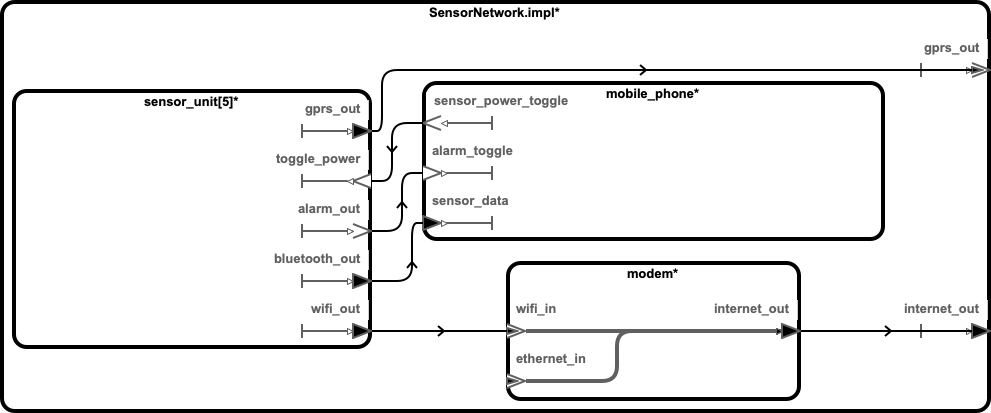
\includegraphics[width=0.9\textwidth]{SensorNetworkAlt}
\end{figure*}

\begin{figure*}[h]
\caption{Internal structure of an alternative Sensor Unit}
\label{fig:sensorunitalt}
\centering
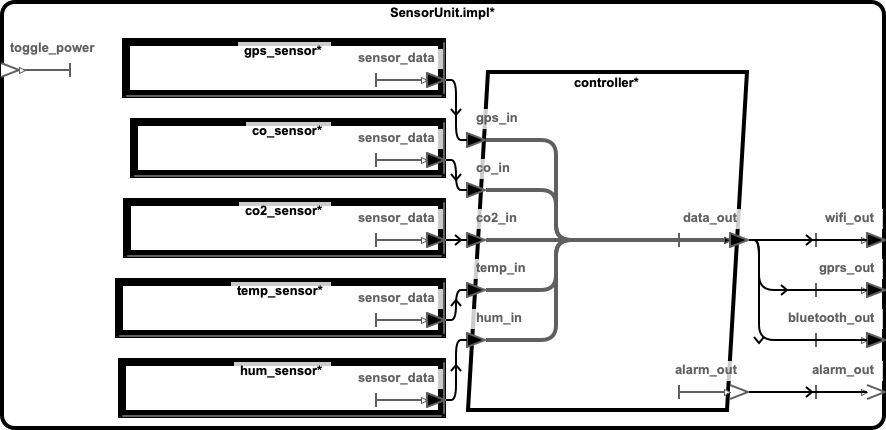
\includegraphics[width=0.9\textwidth]{SensorUnitAlt}
\end{figure*}

\subsection{Architectural Analysis}

Describe how you performed the architectural analysis of the AADL model(s).

\subsection{Results}

Show and discuss the obtained results by provide descriptive statistics and suitable plots.

\limit{6}